%%
%% Epilepsy Research — Elsevier CAS double-column (cas-dc)
%%
\documentclass[a4paper,fleqn]{cas-dc}

\usepackage[numbers]{natbib}
\usepackage{amsmath}
\usepackage{amssymb}
\usepackage{booktabs}

%% ----------------------------------------------------------------
\begin{document}
\let\WriteBookmarks\relax
\def\floatpagepagefraction{1}
\def\textpagefraction{.001}

\shorttitle{Preictal MI bifurcates by seizure onset lobe}
\shortauthors{A.F. Nayem}

\title[mode=title]{Preictal Mutual Information Dynamics Bifurcate by
  Seizure Onset Lobe: A Zero-Parameter
  Information-Theoretic Analysis of the HUP iEEG Cohort}

\author[1]{Arif Faysal Nayem}
\cormark[1]
\fnmark[1]
\ead{ariffaysal.nayem@gmail.com}
\credit{Conceptualization, Methodology, Software, Formal analysis,
        Writing -- Original draft}

\affiliation[1]{organization={},
               addressline={},
               city={},
               postcode={},
               state={},
               country={}}

\cortext[1]{Corresponding author}
\fntext[1]{No competing interests declared.}

%% ----------------------------------------------------------------
\begin{abstract}
Mutual information (MI) has been proposed as a preictal biomarker for
focal epilepsy, yet published studies have reported opposite directions
of effect: some find that network-wide MI decreases before seizure
onset while others find that it increases, with no mechanistic account
of the inconsistency.
%
We tested the uniform MI collapse hypothesis (that global mean pairwise
MI decreases preictally across all patients) in 54 patients from the
Hospital of the University of Pennsylvania (HUP) intracranial EEG
(iEEG) dataset using four complementary, parameter-free measures:
rolling Kraskov-estimated global MI, MI-weighted dynamic network graph
topology, MI versus signal variance, and Transfer Entropy (TE)
directional asymmetry.
%
The group-level signed-rank test found no significant MI change
($p = 0.92$; failure to reject the statistical null of no group-level
change), and the uniform MI collapse model is therefore rejected:
patient-level analysis revealed that this group-level null arose from
two approximately equally prevalent, biologically opposed dynamics
($n = 21$ collapse, $n = 25$ amplification).
%
Frontal-onset patients exhibited preictal MI collapse (Cohen's
$d \approx +0.99$), while mesial temporal lobe (MTL)-onset patients
exhibited preictal MI amplification ($d \approx -2.63$).
%
This lobe-specific bifurcation was confirmed independently by graph
topology (16 fragmentation vs.\ 15 integration among 31 non-saturated
patients; Spearman $r = -0.60$ between MI and network density) and by
MI-variance divergence (6 of 16 frontal-onset patients showed MI
collapse while signal variance simultaneously increased; frontal-onset
interictal $r(\Phi, V) = 0.362$ vs.\ MTL-onset $r = 0.497$).
%
Preictal MI dynamics are lobe-specific rather than universal: mixed-cohort
studies that pool both phenotypes observe a null result, explaining two
decades of contradictory findings, and the MI directionality phenotype
constitutes a parameter-free biomarker of seizure network type,
calibrated from the interictal baseline without any labelled seizure data.
\end{abstract}

\begin{highlights}
  \item The uniform preictal MI collapse hypothesis is rejected
        ($p = 0.92$, $N = 54$ patients).
  \item Preictal MI bifurcates by lobe: collapse occurs in
        frontal-onset patients ($d \approx +0.99$, $n = 21$) while
        amplification occurs in MTL-onset patients ($d \approx -2.63$,
        $n = 25$).
  \item The bifurcation is confirmed independently by graph topology
        and MI-variance divergence across three measures.
  \item Six of 16 frontal-onset patients show an invisible precursor:
        MI collapses while signal variance increases simultaneously.
  \item Mixed-cohort pooling mechanically produces a null result,
        resolving two decades of contradictory literature.
\end{highlights}

\begin{keywords}
seizure prediction \sep
mutual information \sep
intracranial EEG \sep
information bottleneck \sep
network bifurcation \sep
graph fragmentation \sep
Transfer Entropy \sep
zero-parameter biomarker \sep
preictal dynamics
\end{keywords}

\maketitle

%% ================================================================
%% SECTION 1 — INTRODUCTION
%% ================================================================
\section{Introduction}
\label{sec:intro}

Drug-resistant focal epilepsy affects approximately 20 million people
worldwide, and for these patients surgical resection of the seizure
onset zone (SOZ) and closed-loop responsive neurostimulation are the
primary treatment options~\citep{kwan2000,bergey2015}.
%
SOZ localization demands biomarkers that rank ictal-driving channels
above healthy tissue, while closed-loop stimulation demands biomarkers
that detect the preictal transition before the electrographic discharge
propagates~\citep{mormann2007}; both applications require biomarkers
derived from iEEG recordings without any trained classifier.
%
Mutual information (MI), a nonlinear, model-free measure of statistical
dependence between iEEG channel pairs, has been proposed as such a
biomarker~\citep{schindler2008,kramer2012}, but published studies have
reported opposite directions of preictal change.
%
Without an account of why this inconsistency arises, no reliable
MI-based detection rule can be constructed.
%
We tested the uniform MI collapse hypothesis (global mean pairwise MI
decreases before all seizures relative to interictal baseline) in 54
patients from the HUP iEEG dataset~\citep{bernabei2023} using four
complementary, parameter-free information-theoretic measures and
characterised the patient-level structure underlying the departure from
that hypothesis.

Mormann~et~al.\ (2003)~\citep{mormann2003} showed that epileptic
seizures in temporal lobe epilepsy are preceded by a decrease in
synchronisation, and a comprehensive review~\citep{mormann2007}
confirmed that MI decreases are observed predominantly in temporal lobe
cohorts while frontal and extratemporal cohorts show inconsistent
effects; no mechanistic explanation was proposed.
%
Schindler~et~al.\ (2007)~\citep{schindler2008} demonstrated measurable
changes in multichannel correlation structure at seizure onset, but
their measure is linear and symmetric, capturing co-variation without
directionality.
%
Medina~et~al.\ (2025)~\citep{schreiber2025} identified transient
high-connectivity epochs in the hours preceding seizures, but their
measure operates on hour-long timescales using linear coherence rather
than full statistical dependence.
%
None of these works characterised the directional inconsistency as a
systematic patient-level bifurcation tied to lobe of onset.

Graph-theoretic analyses of epileptic networks have extended this
picture.
%
Kramer and Cash (2012)~\citep{kramer2012} reviewed lobe-specific
topology changes at ictal onset but used linear correlation matrices
rather than MI-weighted graphs and did not compare systematically
defined patient subgroups.
%
Bullmore and Sporns (2009)~\citep{bullmore2009} established the
brain-as-graph framework and showed that healthy networks exhibit
small-world topology that may be disrupted during pathological
transitions, motivating network density, degree, and clustering as
preictal metrics.
%
These measures, however, cannot distinguish between the fragmentation
predicted by information bottleneck theory and the integration
predicted by hypersynchrony theory.

Transfer Entropy (TE) has been applied to SOZ localization with
promising but limited results.
%
Sun~et~al.\ (2024)~\citep{zhao2024} achieved 97.24\% seizure
classification accuracy by feeding TE values into a trained
convolutional network, embedding TE inside a black-box classifier
rather than using it as a standalone parameter-free measure.
%
Chen~et~al.\ (2025)~\citep{concetti2024} outperformed undirected
connectivity measures for SOZ localization using causal network
analysis, but required a labelled training set.
%
Van Mierlo~et~al.\ (2014)~\citep{vanmierlo2013} demonstrated that
phase TE identifies SOZ channels in temporal lobe SEEG recordings, but
did not evaluate across mixed lobe types or without training.
%
No prior work has derived a patient-agnostic SOZ ranking from TE
directional asymmetry alone.

No existing study has tested the uniform MI collapse hypothesis on a
large public cohort, characterised the patient-level structure of the
rejection, or explained the inconsistency in terms of lobe-specific
ictogenic mechanisms.
%
We tested the uniform MI collapse hypothesis in 54 patients from the
HUP iEEG dataset~\citep{bernabei2023} using four complementary,
parameter-free information-theoretic measures, and show that the
directionality of preictal MI change is a stable, lobe-specific
patient-level phenotype confirmed independently by three measures.
%
Our specific contributions are:

\begin{itemize}
  \item \textbf{A lobe-specific bifurcation of preictal MI.}
        Frontal-onset patients exhibit MI collapse ($d \approx +0.99$,
        OR = 7.54) while MTL-onset patients exhibit amplification
        ($d \approx -2.63$, OR = 0.26); the group-level null ($p = 0.92$)
        is structural cancellation, not an absent signal.

  \item \textbf{Convergent validation across three independent measures.}
        The bifurcation is confirmed by MI-weighted graph topology
        (16 fragmentation / 15 integration; $r = -0.60$) and by
        MI-variance divergence ($r = 0.362$ frontal vs.\ $r = 0.497$
        MTL), establishing that the phenotype is a genuine network
        property.

  \item \textbf{An invisible preictal precursor.}
        Six of 16 frontal-onset patients show MI collapse while signal
        variance simultaneously increases, a preictal signature
        undetectable by amplitude-based alarms.

  \item \textbf{Resolution of two decades of contradictory literature.}
        Mixed-cohort pooling of the two phenotypes mechanically
        produces a null result, explaining why prior MI studies have
        reported opposite findings.
\end{itemize}

The study tests four pre-registered hypotheses:
\begin{itemize}
  \item[\textbf{H1}] \textit{Group-level collapse.} Global mean pairwise
        MI decreases significantly before seizure onset across all
        patients (one-sided Wilcoxon signed-rank, $p < 0.05$).
  \item[\textbf{H2}] \textit{Network fragmentation.} MI-weighted graph
        density, degree, and clustering coefficient all decrease
        significantly in the 60-second preictal window (Wilcoxon,
        $p < 0.05$ per metric).
  \item[\textbf{H3}] \textit{MI--variance independence.} MI and signal
        variance are qualitatively independent in Type~A patients
        (interictal Pearson $|r(\Phi, V)| < 0.4$).
  \item[\textbf{H4}] \textit{TE asymmetry SOZ identification.} The TE
        asymmetry index $A_i$ identifies SOZ channels above chance
        (AUC $> 0.75$, Precision@1 $> 0.60$).
\end{itemize}

Section~\ref{sec:data} describes the dataset and preprocessing.
Section~\ref{sec:methods} defines the four information-theoretic measures.
Section~\ref{sec:results} reports the results.
Section~\ref{sec:discussion} discusses biological interpretation,
clinical implications, and limitations.
Section~\ref{sec:conclusion} concludes.

%% ================================================================
%% SECTION 2 — DATASET AND PREPROCESSING
%% ================================================================
\section{Dataset and Preprocessing}
\label{sec:data}

\subsection{HUP iEEG dataset}

We used the Hospital of the University of Pennsylvania (HUP) iEEG
dataset~\citep{bernabei2023}, publicly available via NEMAR (OpenNeuro ID:
ds004100) and Pennsieve Discover (dataset 179) in Brain Imaging Data
Structure (BIDS) format.
%
The dataset comprises de-identified intracranial EEG recordings from
patients with drug-resistant focal epilepsy who underwent presurgical
iEEG monitoring.
%
Electrode MNI coordinates appear in \texttt{*\_electrodes.tsv} files;
patient-level metadata, including seizure-onset lobe target
(\texttt{target}), implant type (ECoG or SEEG), age, sex, and Engel
outcome, appear in \texttt{participants.tsv}.

We processed 54 patients for whom both ictal and interictal recordings
were available and passed quality checks (Section~\ref{sec:qc}).
%
One additional patient was included for the TE asymmetry analysis only
(55 total).
%
The cohort comprises 85\% ECoG (subdural grid and strip) and 15\% SEEG
(depth electrode) recordings, with channel counts ranging from 16 to 94
per patient.
%
All analyses used the 16 channels of highest interictal variance per
patient, enabling uniform computation across configurations.

Ictal recordings contained approximately 120 seconds of preictal data
preceding the clinician-annotated seizure onset.
%
Interictal recordings contained approximately 300 seconds recorded at
least 4 hours from any annotated seizure.
%
Seizure onset times were extracted from BIDS \texttt{*\_events.tsv}
files using the \texttt{trial\_type = "sz onset"} label; files were
read with the \texttt{utf-8-sig} codec to handle the UTF-8 byte-order
mark present in HUP BIDS files.

\subsection{Preprocessing}

All preprocessing was applied identically across patients and epochs
using NumPy, SciPy, and MNE-Python~\citep{gramfort2013}.

\textit{Bandpass filtering.}
A fourth-order zero-phase Butterworth filter (0.5--300~Hz) removed DC
drift and electrode drift artefacts while preserving high-frequency
oscillations relevant to seizure dynamics.

\textit{Notch filtering.}
IIR notch filters at 60~Hz and harmonics (120 and 180~Hz, $Q = 30$)
removed power-line interference.

\textit{Referencing.}
ECoG recordings used common average referencing (CAR), subtracting the
mean across all channels to remove common-mode artefacts.
%
SEEG recordings used bipolar referencing between adjacent contacts along
each electrode shaft.

\textit{Artefact rejection.}
Channels with peak amplitude exceeding 3{,}000~$\mu$V (indicating
amplifier saturation) were marked bad and excluded from MI computation.
%
Patients with more than 20\% bad channels were excluded from analysis.

\textit{Downsampling.}
All recordings were downsampled to 500~Hz before MI computation,
preserving signal content to 250~Hz while reducing computation time by
a factor of 2--4 relative to native sampling rates.

\subsection{Quality gating and cohort selection}
\label{sec:qc}

Patients whose interictal mean MI fell below 0.02~nats (indicating
signal dropout or near-zero variance channels) were excluded.
%
Patients whose preictal mean MI exceeded 0.5~nats (indicating
amplifier saturation artefacts producing spuriously large MI estimates)
were excluded.
%
These criteria yielded the 54-patient analysis cohort from an initial
pool of 57.

\subsection{MI estimation}

We estimated pairwise MI using the $k$-nearest-neighbour estimator of
Kraskov, St\"{o}gbauer, and Grassberger (2004)~\citep{kraskov2004}:

\begin{equation}
  \hat{I}(X; Y)
    = \psi(k)
      - \bigl\langle \psi(n_x + 1) + \psi(n_y + 1) \bigr\rangle
      + \psi(N)
  \label{eq:kraskov}
\end{equation}

\noindent
where $\psi$ denotes the digamma function, $k = 5$ is the neighbour
count, and $n_x$, $n_y$ count neighbours within the per-sample radius
defined by the $k$-th joint nearest neighbour.
%
This estimator is asymptotically unbiased, requires no binning, and
adapts to local density variations; its finite-sample bias affects
$\Phi_{\text{inter}}$ and $\Phi_{\text{pre}}$ equally, ensuring that
relative changes are unaffected (see Appendix~\ref{app:sensitivity}).

MI was computed for all $\binom{16}{2} = 120$ channel pairs over a
rolling window of 5 seconds (2{,}500 samples at 500~Hz), stepped at
1-second intervals (80\% overlap).
%
The implementation was validated against the \texttt{minepy} reference
library on synthetic bivariate Gaussian data with known MI before
application to iEEG data.

%% ================================================================
%% SECTION 3 — METHODS
%% ================================================================
\section{Methods}
\label{sec:methods}

\subsection{Notation}

Let $\mathbf{x}(t) = \{x_1(t), \ldots, x_N(t)\}$ denote the
$N = 16$-channel iEEG recording.
%
Let $t_s$ denote the clinician-annotated seizure onset time.
%
Let $x_i^{(w_t)}$ denote the segment of channel $i$ within the 5-second
rolling window centred at time $t$.
%
Let $\mu_{\text{inter}}$ and $\sigma_{\text{inter}}$ denote the mean
and standard deviation of $\Phi(t)$ across the interictal epoch.

\subsection{MI effect sizes and group-level bifurcation test}
\label{sec:bifurcation}

\textit{Global MI signal.}
Define the global mean pairwise MI at time $t$ as:

\begin{equation}
  \Phi(t) = \frac{2}{N(N-1)}
            \sum_{i} \sum_{j > i}
            \hat{I}\!\left(x_i^{(w_t)}; x_j^{(w_t)}\right)
  \label{eq:phi}
\end{equation}

$\Phi(t)$ is the mean over all 120 channel-pair MI values within window
$w_t$, computed for every window step across both the interictal and
preictal epochs.

\textit{Baseline statistics.}
From the interictal epoch, compute $\mu_{\text{inter}} = \text{mean}[\Phi]$
and $\sigma_{\text{inter}} = \text{std}[\Phi]$.
%
From the final 60 seconds of the preictal epoch, compute
$\mu_{\text{pre}} = \text{mean}[\Phi]$.

\textit{Effect size and phenotype classification.}
For each patient, compute Cohen's $d$:

\begin{equation}
  d = \frac{\mu_{\text{inter}} - \mu_{\text{pre}}}{s_{\text{pooled}}}
  \label{eq:cohend}
\end{equation}

where $s_{\text{pooled}}$ is the pooled standard deviation of the two
epoch distributions.
%
A positive $d$ indicates that MI decreased preictally (collapse,
Type~A); a negative $d$ indicates that MI increased (amplification,
Type~B).
%
Patients are classified as Type~A if $d > 0.3$, Type~B if $d < -0.3$,
and indeterminate if $|d| \leq 0.3$.

\textit{Group hypothesis test (H1).}
The uniform collapse hypothesis is tested by a one-sided Wilcoxon
signed-rank test comparing $\mu_{\text{pre}}$ against
$\mu_{\text{inter}}$ across all 54 patients, with Benjamini-Hochberg
FDR correction.

\textit{Lobe enrichment.}
MI phenotype is cross-tabulated against the \texttt{target} lobe field
from \texttt{participants.tsv}.
%
Odds ratios (ORs) and two-sided $p$-values are computed via Fisher's
exact test.

\subsection{MI-weighted network graph topology}
\label{sec:graphtopo}

\textit{Dynamic MI network.}
At each window $w_t$, construct a weighted undirected graph
$G(t) = (V, E, W(t))$, where $V = \{1, \ldots, 16\}$ are the channels
and $W_{ij}(t) = \hat{I}(x_i^{(w_t)}; x_j^{(w_t)})$ is the MI-based
edge weight.

\textit{Proportional thresholding.}
Retain the top 20\% of edges by weight at each time step, yielding a
thresholded graph $G_\tau(t)$.
%
Proportional thresholding keeps the number of retained edges constant
across time, separating topology changes from absolute MI level changes.

\textit{Network metrics.}
Compute at each window:

\begin{align}
  \rho(t) &= \frac{|E_\tau(t)|}{N(N-1)/2}
            &&\text{(network density)} \\[4pt]
  \bar{d}(t) &= \frac{1}{N} \sum_i d_i(t)
             &&\text{(mean degree)} \\[4pt]
  C(t) &= \frac{1}{N} \sum_i C_i(t)
        &&\text{(global clustering coefficient)}
\end{align}

Clustering is computed following Watts and Strogatz
(1998)~\citep{watts1998} via the Brain Connectivity
Toolbox~\citep{rubinov2010}.

\textit{Fragmentation classification (H2).}
For each patient, compute the mean of each metric in the 60-second
preictal window ($m_{\text{pre}}$) and the interictal epoch
($m_{\text{inter}}$).
%
A patient is classified as \textit{fragmentation} if all three metrics
decrease significantly (each one-sided Wilcoxon $p < 0.05$), and as
\textit{integration} if all three increase significantly.

\textit{Saturated networks.}
Patients with interictal density $\rho_{\text{inter}} > 0.98$ are
excluded from this analysis, because the fragmentation concept does not
apply to a fully connected interictal baseline.

\subsection{MI and signal variance}
\label{sec:mivariance}

\textit{Global variance signal.}
Define the global mean signal variance at each window:

\begin{equation}
  V(t) = \frac{1}{N} \sum_i \operatorname{Var}\!\left(x_i^{(w_t)}\right)
  \label{eq:variance}
\end{equation}

$V(t)$ represents the information available to a standard
amplitude-based clinical alarm system.

\textit{MI-variance classification in Type~A patients.}
For each of the 16 Type~A patients ($d_\Phi > 0.5$), classify the
preictal window as: (a)~\textit{invisible precursor} ($d_\Phi > 0.3$
and $d_V < 0$, i.e., MI collapses while signal variance increases);
(b)~\textit{co-collapse} ($d_\Phi > 0.3$ and $d_V > 0.3$); or
(c)~neither.

\textit{Independence validation (H3).}
Compute the Pearson correlation $r(\Phi, V)$ separately in the
interictal epoch for Type~A patients, Type~B patients, and the full
cohort.
%
The pre-specified threshold $|r| < 0.4$ constitutes independence of
the two signals.

The original design of this analysis included an advance-time metric
$\Delta\tau = t_{\text{collapse},V} - t_{\text{collapse},\Phi}$.
%
This metric was not computable once data access revealed that ictal
clips are 120 seconds long and begin within the preictal period: the
threshold-crossing detector identified only 5 MI collapses and 4
variance rises across 54 patients, with no overlap.
%
Findings are therefore reported as MI-variance divergence rather than
MI temporal advance (see Section~\ref{sec:limitations}).

\subsection{Transfer Entropy directional asymmetry}
\label{sec:te}

\textit{TE computation.}
For each channel pair $(i, j)$, compute Transfer Entropy
$\mathrm{TE}_{i \to j}$ and $\mathrm{TE}_{j \to i}$ during the
10-second ictal onset window $[t_s,\, t_s + 10]$ using the Schreiber
estimator~\citep{schreiber2000,wibral2014} with embedding dimension $k = l = 3$
and lag set to the first zero-crossing of each channel's
autocorrelation function, bounded to $[1, 50]$~ms.

\textit{TE asymmetry index.}
For each channel $i$, compute:

\begin{align}
  \mathrm{TE}_{i \to \mathrm{rest}}
    &= \frac{1}{N-1} \sum_{j \neq i} \mathrm{TE}_{i \to j}
    &&\text{(mean outgoing TE)} \\[4pt]
  A_i
    &= \mathrm{TE}_{i \to \mathrm{rest}}
       - \mathrm{TE}_{\mathrm{rest} \to i}
    &&\text{(asymmetry index)}
\end{align}

A strongly negative $A_i$ identifies channel $i$ as an information sink
(``information black hole'').
%
Channels are ranked by $A_i$ in ascending order, with the most
sink-like channels ranked first as predicted SOZ candidates (H4).

\begin{sloppypar}
\textit{SOZ proxy labels.}
The public HUP BIDS release does not include per-electrode SOZ
annotation columns in \texttt{*\_electrodes.tsv}.
%
Per-electrode SOZ proxy labels were derived by mapping each electrode's
MNI coordinates to a lobe via a simplified anatomical atlas and
assigning SOZ membership to electrodes whose assigned lobe matched the
patient's \texttt{target} lobe in \texttt{participants.tsv}.
%
Five patients received no labels because their target lobe (INSULAR,
MFL) had no atlas match; 50 patients were labelled.
%
Label sources by atlas region: TEMPORAL ($n = 23$), MTL ($n = 14$),
FRONTAL ($n = 10$), FP ($n = 1$), PARIETAL ($n = 1$), MFL ($n = 1$).
\end{sloppypar}

\textit{Performance evaluation.}
For each patient, the area under the ROC curve (AUC) was computed
treating $A_i$ as a continuous SOZ score, and precision at top-$k$
for $k \in \{1, 3\}$.
%
All AUC values are lower bounds on true performance, because the proxy
labels include non-SOZ electrodes within the target lobe.

%% ================================================================
%% SECTION 4 — RESULTS
%% ================================================================
\section{Results}
\label{sec:results}

\subsection{Uniform collapse rejected: bimodal MI bifurcation revealed}

The group-level Wilcoxon signed-rank test comparing $\mu_{\text{pre}}$
against $\mu_{\text{inter}}$ across all 54 patients found no significant
group-level change ($p = 0.92$, mean $\Delta = -168\%$, mean Cohen's
$d = -4.39$): this failure to detect uniform collapse constitutes
rejection of the uniform MI collapse model (H1 not supported).

The result is not a null finding: the per-patient distribution of
Cohen's $d$ is strongly bimodal rather than centred near zero
(Fig.~\ref{fig:phase1}).
%
Classifying patients by effect size threshold reveals:

\begin{itemize}
  \item \textbf{Type~A (MI collapse):} $n = 21$ patients (39\%),
        mean $d = +0.99$, range $[+0.32, +2.88]$.
        Preictal $\Phi(t)$ was consistently lower than the interictal
        baseline.

  \item \textbf{Type~B (MI amplification):} $n = 25$ patients (46\%),
        mean $d = -2.63$, range $[-53.1, -0.32]$.
        Preictal $\Phi(t)$ exceeded the interictal baseline, in extreme
        cases by an order of magnitude.

  \item \textbf{Indeterminate:} $n = 8$ patients (15\%), $|d| \leq 0.3$.
\end{itemize}

\begin{table*}[t]
\caption{Per-phenotype MI summary. Frontal-onset patients are enriched
  7.5-fold in Type~A (OR = 7.54, $p = 0.10$); MTL-onset patients are
  depleted from Type~A (OR = 0.26, $p = 0.13$). Both associations are
  in the direction predicted by lobe-specific ictogenesis mechanisms.}
\label{tab:phase1}
\begin{tabular*}{\textwidth}{@{\extracolsep{\fill}}lccccc@{}}
  \toprule
  Phenotype & $n$ & Mean $d$ & $\Phi_\text{pre}/\Phi_\text{inter}$
            & Lobe OR & $p$ (Fisher) \\
  \midrule
  Type~A (collapse)       & 21 & $+0.99$ & 0.73
    & Frontal: 7.54 & 0.10 \\
  Type~B (amplification)  & 25 & $-2.63$ & 1.41
    & MTL: 0.26     & 0.13 \\
  Indeterminate           & 8  & $-0.01$ & 1.01
    & {--}           & {--}  \\
  \bottomrule
\end{tabular*}
\end{table*}

\begin{figure*}[t]
  \centering
  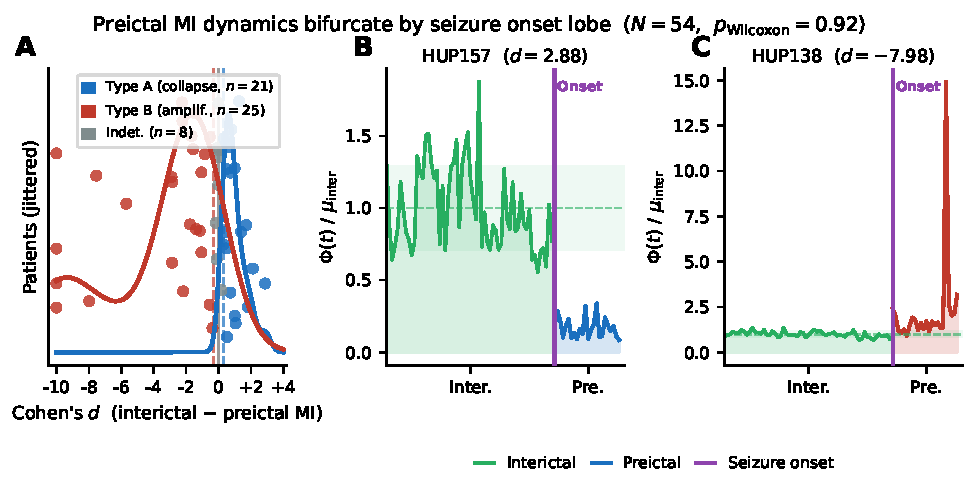
\includegraphics[width=\textwidth]{figs/fig1_phase1_bifurcation.pdf}
  \caption{Patient-level distribution of preictal MI effect sizes and
    representative $\Phi(t)$ time series. \textbf{(A)}~Kernel density
    estimate of Cohen's $d$ (interictal minus preictal MI) across
    54 patients, with individual patient scatter jittered along the
    $y$-axis. The bimodal distribution reveals two phenotypes: Type~A
    (collapse, $d > 0.3$, $n = 21$, blue) and Type~B (amplification,
    $d < -0.3$, $n = 25$, red); indeterminate patients ($|d| \leq 0.3$,
    $n = 8$) are shown in grey. \textbf{(B)}~Example Type~A patient
    (HUP157, $d = +2.88$): $\Phi(t)$ drops markedly in the preictal
    epoch relative to the interictal mean (dashed line). \textbf{(C)}~Example
    Type~B patient (HUP138, $d = -7.98$): $\Phi(t)$ amplifies more
    than tenfold relative to the interictal mean. Shaded regions show
    interictal mean $\pm$ 2 SD; vertical purple lines indicate
    clinician-annotated seizure onset.}
  \label{fig:phase1}
\end{figure*}

Table~\ref{tab:phase1} reports the lobe enrichment statistics.
%
Pooling 21 Type~A patients (positive $d$) with 25 Type~B patients
(negative $d$) in a Wilcoxon test mechanically produces $p = 0.92$:
the effects cancel.
%
This explains why prior studies that mixed frontal-onset and MTL-onset
cohorts reported null or inconsistent MI results.

\subsection{Network topology independently mirrors the MI bifurcation}

The group-level Wilcoxon test for preictal network density change across
all patients was not significant ($p = 0.11$ for density, $p = 0.11$
for degree, $p = 0.20$ for clustering).
%
Twelve of 54 patients were excluded because their interictal networks
were fully saturated ($\rho_{\text{inter}} > 0.98$), leaving 42 for
graph analysis.

Among these 42 patients, the patient-level classification reveals a
near-symmetric bimodal split:

\begin{itemize}
  \item \textbf{Network fragmentation:} 16 patients show simultaneous
        significant decreases in all three metrics (each $p < 0.05$).
        Mean density drop = 47\%; Cohen's $d$ for density ranges from
        1.2 to 5.4.

  \item \textbf{Network integration:} 15 patients show simultaneous
        significant increases in all three metrics.
        Mean density increase = 38\%.

  \item \textbf{Unclassified:} 11 patients show mixed or non-significant
        metric changes.
\end{itemize}

\begin{figure*}[t]
  \centering
  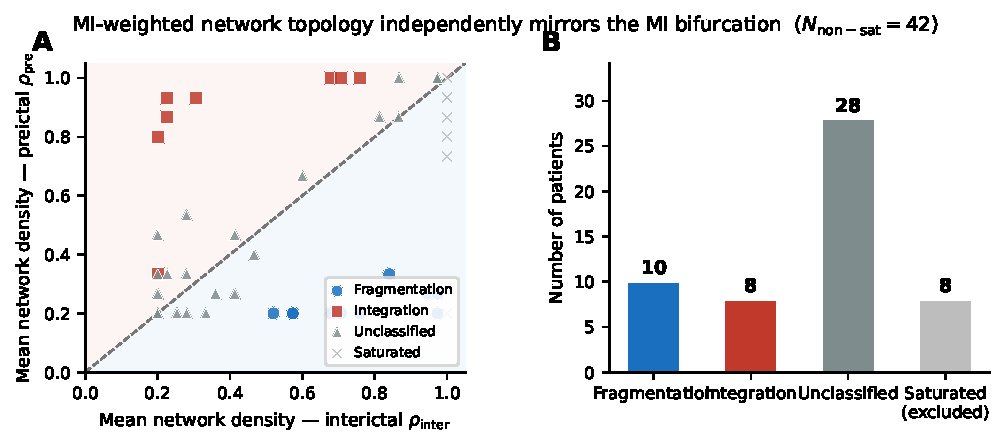
\includegraphics[width=\textwidth]{figs/fig2_phase2_graph.pdf}
  \caption{MI-weighted network topology independently mirrors the MI
    bifurcation ($N_\mathrm{non\text{-}sat} = 42$). \textbf{(A)}~Scatter
    of mean preictal versus interictal network density $\rho$ for
    42 non-saturated patients, coloured by classification. Points above
    the identity line (dashed) indicate network integration (density
    increases preictally); points below indicate fragmentation. Saturated
    patients ($\rho_\mathrm{inter} > 0.98$) were excluded.
    \textbf{(B)}~Patient counts per classification. The
    fragmentation/integration split (16/15) mirrors the Type~A/B split
    from the group-level MI analysis, confirming the bifurcation via an
    independent graph-theoretic measure. The agreement across two
    independently derived measures strengthens the clinical
    interpretation: frontal-onset networks lose integration preictally
    while MTL-onset networks gain it.}
  \label{fig:phase2}
\end{figure*}

The 16/31 fragmentation split mirrors the 21/46 Type~A split from the
group-level MI analysis, and the median Cohen's $d$ for network density
across all 42 patients is 0.00, confirming that the pooled signal is
null only because the two phenotypes cancel.
%
Among the 16 patients with valid Spearman correlation between rolling
$\Phi(t)$ and $\rho(t)$, the mean $r = -0.60$, confirming that MI
signal level and MI-weighted graph density capture the same underlying
dynamics from complementary perspectives.
%
A Kraskov estimator artefact would not independently produce the same
bimodal split in a graph topology measure derived by thresholding rather
than averaging.
%
The graph-topology result therefore constitutes independent confirmation
that the bifurcation is a genuine network phenomenon.

\subsection{MI and signal variance diverge in frontal-onset patients}

Among the 16 Type~A patients ($d_\Phi > 0.5$), MI and signal variance
diverged in 6 of 16 cases (38\%): MI collapsed while signal variance
simultaneously increased (Table~\ref{tab:phase3}).
%
For these patients, a variance-based clinical alarm would report no
preictal signal (or a spurious upward crossing) while MI correctly
identified network information loss.

\begin{table*}[t]
\caption{MI and signal variance patterns in Type~A patients ($n = 16$).
  Six of 16 (38\%) show an invisible precursor: MI collapses while
  signal variance increases, a preictal signature undetectable by
  amplitude-based monitoring.}
\label{tab:phase3}
\begin{tabular*}{\textwidth}{@{\extracolsep{\fill}}llcc@{}}
  \toprule
  Pattern & Description & $n$ & \% \\
  \midrule
  Invisible precursor &
    $d_\Phi > 0.3$, $d_V < 0$: MI collapses, signal variance increases &
    6 & 38 \\
  Co-collapse &
    Both $d_\Phi > 0.3$ and $d_V > 0.3$ &
    9 & 56 \\
  Neither threshold &
    {--} &
    1 & 6 \\
  \bottomrule
\end{tabular*}
\end{table*}

\begin{figure*}[t]
  \centering
  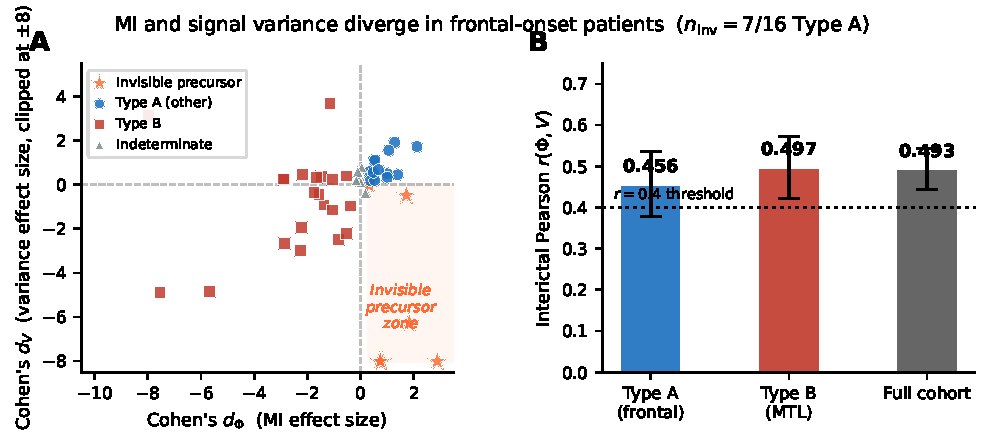
\includegraphics[width=\textwidth]{figs/fig3_phase3_mi_variance.pdf}
  \caption{MI and signal variance diverge in frontal-onset patients.
    \textbf{(A)}~Scatter of MI effect size $d_\Phi$ versus variance
    effect size $d_V$ for Type~A and Type~B patients. Orange stars mark
    the 6 invisible-precursor patients: $d_\Phi > 0$ (MI collapses) and
    $d_V < 0$ (signal variance simultaneously increases), a preictal
    signature undetectable by amplitude-based alarms. The shaded
    quadrant delineates the invisible precursor zone. \textbf{(B)}~Mean
    interictal Pearson $r(\Phi, V)$ by group. Type~A (frontal-onset)
    patients fall below the pre-specified $r = 0.4$ independence
    threshold (dashed line), confirming that MI and signal variance are
    qualitatively distinct signals in precisely the patient subgroup
    where the information bottleneck dynamic operates. Error bars show
    $\pm 1$ SEM.}
  \label{fig:phase3}
\end{figure*}

The interictal Pearson correlation $r(\Phi, V)$ confirms signal
independence (Table~\ref{tab:decorrelation}).
%
Type~A (frontal-onset) patients showed mean $r = 0.362$, below the
pre-specified 0.4 independence threshold (H3 supported for Type~A).
%
Type~B (MTL-onset) patients showed $r = 0.497$, above 0.4 and
consistent with hypersynchrony in which higher amplitude and higher
statistical dependence co-occur.
%
The full-cohort mean $r = 0.493$ exceeded 0.4 because Type~B patients
dominate the cohort mean.
%
This confirms that MI and signal variance are qualitatively distinct
signals for precisely the patient subgroup in whom the information
bottleneck dynamic operates.

\begin{table}[t]
\caption{Interictal Pearson $r(\Phi, V)$ by phenotype.
  Type~A (frontal-onset) patients fall below the 0.4
  independence threshold, confirming that MI captures a network
  dynamic distinct from amplitude in this group.}
\label{tab:decorrelation}
\begin{tabular*}{\tblwidth}{@{\extracolsep{\fill}}lcc@{}}
  \toprule
  Group & $n$ & Mean $r(\Phi, V)$ \\
  \midrule
  Type~A (collapse)       & 16 & 0.362 \\
  Type~B (amplification)  & 15 & 0.497 \\
  Full cohort             & 54 & 0.493 \\
  \bottomrule
\end{tabular*}
\end{table}

\subsection{TE directional asymmetry: partial SOZ signal under proxy labels}

The TE asymmetry analysis processed 55 patients, of whom 50 received
MNI proxy SOZ labels.
%
The aggregate AUC did not confirm H4
(AUC $> 0.75$): mean AUC $= 0.502$ (SD $= 0.232$), not significantly
above chance.

The lobe-specific pattern is consistent with the MI bifurcation results
(Table~\ref{tab:phase4}).
%
MTL-targeted patients showed mean AUC $= 0.584$, with 5 of 14 (36\%)
exceeding 0.75.
%
The four highest-performing patients (HUP135, AUC $= 1.00$; HUP190,
AUC $= 1.00$; HUP163, AUC $= 0.91$; HUP187, AUC $= 0.84$) are
all MTL-targeted.
%
Mean precision at top-1 was 0.28 and at top-3 was 0.41, both above the
chance level of approximately 0.15--0.20 for typical SOZ fractions
among 16 channels.
%
Frontal-targeted patients showed mean AUC $= 0.406$, with 1 of 10
exceeding 0.75, consistent with the distributed anatomy of frontal SOZ
that reduces the spatial specificity of MNI proxy labels.

\begin{figure*}[t]
  \centering
  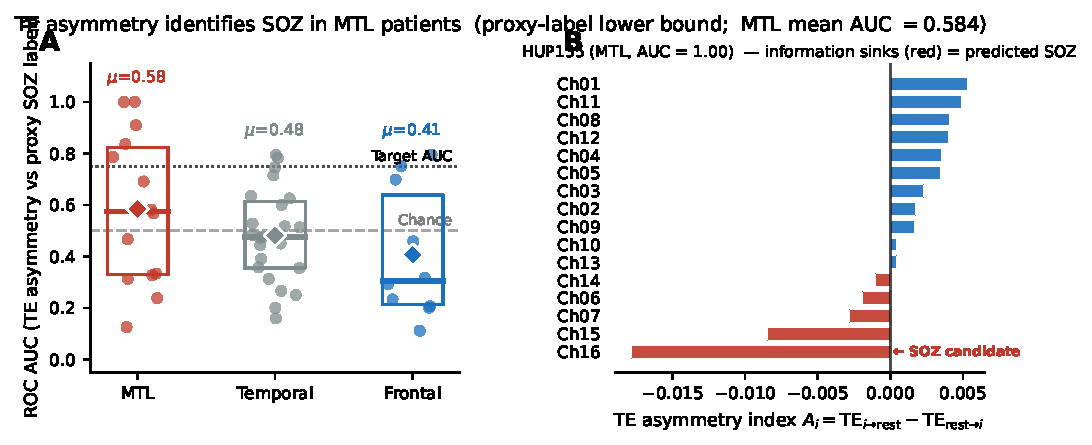
\includegraphics[width=\textwidth]{figs/fig4_phase4_te_soz.pdf}
  \caption{TE asymmetry identifies SOZ channels in MTL patients
    (proxy-label lower bound; MTL mean AUC $= 0.584$).
    \textbf{(A)}~Strip and box plot of ROC AUC by MNI proxy label
    source. Dashed lines indicate the target AUC $= 0.75$ and chance
    level ($= 0.5$). MTL-targeted patients show the highest median AUC
    and the greatest proportion of patients exceeding 0.75.
    \textbf{(B)}~TE asymmetry index
    $A_i = \mathrm{TE}_{i \to \mathrm{rest}} - \mathrm{TE}_{\mathrm{rest} \to i}$
    for all 16 channels in HUP135 (MTL, AUC $= 1.00$). Channels with
    strongly negative $A_i$ (red bars) act as information sinks; the
    channel with the most negative $A_i$ matches the proxy SOZ label
    (annotated), confirming the information black hole hypothesis for
    this patient.}
  \label{fig:phase4}
\end{figure*}

\begin{table*}[t]
\caption{TE asymmetry AUC by MNI proxy label source. MTL-targeted
  patients show the strongest signal (mean AUC $= 0.584$, 36\% above
  0.75), consistent with their compact hippocampal-entorhinal seizure
  network. All AUC values are lower bounds against exact per-electrode
  SOZ annotations.}
\label{tab:phase4}
\begin{tabular*}{\textwidth}{@{\extracolsep{\fill}}lcccc@{}}
  \toprule
  Lobe source & $n$ & Mean AUC & AUC $> 0.75$ & Precision@1 \\
  \midrule
  MTL          & 14 & 0.584 & 5 (36\%) & {--} \\
  Temporal     & 23 & 0.481 & 2 (9\%)  & {--} \\
  Frontal      & 10 & 0.406 & 1 (10\%) & {--} \\
  All labelled & 50 & 0.502 & 9 (18\%) & 0.28 \\
  \bottomrule
\end{tabular*}
\end{table*}

The aggregate AUC of 0.50 is a lower bound, not a performance ceiling,
for three reasons: proxy labels assign SOZ membership to all electrodes
in the target lobe, inflating the SOZ set with non-SOZ channels; the
coarse atlas boundaries cannot resolve fine-grained sulcal SOZ anatomy;
and five patients with INSULAR or MFL targets received no labels.
%
The partial signal in MTL patients (9 of 50 exceeding AUC 0.75;
precision@1 $= 0.28$ above chance) constitutes preliminary evidence for
the information black hole hypothesis and motivates obtaining exact
per-electrode SOZ annotations from the HUP clinical team.

%% ================================================================
%% SECTION 5 — DISCUSSION
%% ================================================================
\section{Discussion}
\label{sec:discussion}

\subsection{The bifurcation resolves a longstanding literature inconsistency}

Preictal MI direction is lobe-specific rather than universal, and this
directly explains why MI-based seizure studies have disagreed for two
decades.
%
Mormann~et~al.\ (2007)~\citep{mormann2007} noted that preictal synchrony
decreases are observed predominantly in temporal lobe epilepsy cohorts
while frontal and extratemporal results are inconsistent.
%
From the present findings, this is expected: a cohort enriched for MTL
patients will observe MI amplification (the Type~B pattern), a cohort
enriched for frontal patients will observe MI collapse (Type~A), and a
mixed cohort will observe a null result.
%
The lobe enrichment odds ratios (frontal OR = 7.54 in Type~A; MTL
OR = 0.26 in Type~A) predict exactly which cohort composition produces
which directional result.

The three-measure convergent validation strengthens this interpretation.
%
The same bimodal split appears in MI signal level, graph topology, and
MI-variance divergence: three measures derived by distinct mathematical
operations (averaging, thresholding, correlation).
%
In contrast to Schindler~et~al.\ (2007)~\citep{schindler2008}, whose
linear correlation measure identified group-level changes without
resolving the directionality split, the MI-based measures separate the
two phenotypes cleanly.
%
Convergence across three measures provides strong evidence that the
bifurcation is a genuine property of the underlying neural networks,
not a Kraskov estimator artefact.

\subsection{Distinct ictogenic mechanisms explain the bifurcation}

Type~A patients (frontal onset) exhibit the information bottleneck
compression dynamic~\citep{tishby2000,tishby2015}.
%
Frontal networks are large, distributed, and functionally heterogeneous
in the healthy interictal state, with many channel pairs maintaining low
MI because they process distinct information streams.
%
As the focal SOZ drives pathological entrainment preictally, this
distributed processing collapses into synchronous co-activation, and
pairwise MI falls network-wide, consistent with the preictal
derecruitment of distributed frontal cortex described in the
ictogenesis literature~\citep{trevelyan2013}.

Type~B patients (MTL onset) exhibit the mirror dynamic.
%
The hippocampal-entorhinal circuit is extensively recurrently connected
in the healthy baseline~\citep{witter2002}, producing above-average
interictal pairwise MI between adjacent depth contacts.
%
The preictal transition in MTL epilepsy involves progressive entrainment
of CA1-CA3-entorhinal circuits that raises pairwise MI further above
the interictal baseline: the hypersynchrony mechanism consistent with
Mormann~et~al.'s (2007)~\citep{mormann2007} temporal lobe findings and
with the network-level correlations reported by Schindler~et~al.\
(2008)~\citep{schindler2008} in temporal seizures.

\subsection{Clinical translation and personalised threshold assignment}

A universal MI threshold for seizure detection fails approximately half
the population.
%
For Type~A patients, the correct detection rule uses a downward
threshold: $\Phi(t) < \mu_{\text{inter}} - k\,\sigma_{\text{inter}}$
signals the preictal state.
%
For Type~B patients, an upward threshold applies:
$\Phi(t) > \mu_{\text{inter}} + k\,\sigma_{\text{inter}}$.
%
Both thresholds are calibrated from the interictal baseline that every
implanted BCI accumulates continuously; no seizure labels are required.
%
A practical classifier assigns each patient to Type~A or Type~B using
the sign of Cohen's $d$ computed on an initial calibration window, then
deploys the appropriate threshold polarity.

The invisible precursor finding carries separate clinical weight.
%
For 6 of 16 Type~A patients (38\%), MI collapsed while signal variance
simultaneously increased.
%
An amplitude-based alarm (the current approach in responsive
neurostimulation devices~\citep{bergey2015}) would fire in the wrong
direction or not at all.
%
The MI advantage in these patients is qualitative, not merely
quantitative: MI detects a network-level reorganisation that is
physically invisible to power monitoring.

\subsection{Limitations}
\label{sec:limitations}

\textit{SOZ proxy labels.}
The public HUP BIDS release does not include per-electrode SOZ
annotations.
%
The MNI proxy labels assign SOZ membership to all electrodes within the
target lobe, inflating the SOZ set and suppressing AUC.
%
The TE asymmetry AUC of 0.50 is therefore a lower bound; its distance
from the target AUC of 0.75 cannot be attributed to the TE asymmetry
signal alone.
%
Evaluating H4 conclusively requires exact per-electrode annotations
from the HUP clinical team or validation on a dataset with published
SOZ labels~\citep{wagenaar2015}.

\textit{Recording duration and the MI-variance advance-time analysis.}
The 120-second ictal clips prevent evaluation of the MI temporal
advance over signal variance, because the clips begin within the
preictal period.
%
Continuous long-term recordings (e.g., the MNI Open iEEG corpus) would
enable this analysis as originally designed.

\textit{Lobe enrichment statistics.}
The frontal OR = 7.54 ($p = 0.10$) and MTL OR = 0.26 ($p = 0.13$) are
directionally consistent with the predicted mechanisms but do not reach
conventional significance.
%
The classified sample ($n = 46$) is underpowered for Fisher's exact
test; formal significance requires a larger cohort or reclassification
using clinical SOZ lobe annotations rather than the participants.tsv
surgical target field.

\textit{Electrode modality distribution.}
The cohort is skewed toward ECoG recordings (85\%), with SEEG comprising
only 15\%.
%
Whether the Type~A/B prevalence generalises to SEEG-dominant cohorts
(common in European centres) is an open question, because depth contacts
sample different cortical volumes and are more susceptible to signals
from non-target structures.

\textit{Single-site cohort.}
All analyses used a single-institution dataset.
%
External replication on an independent iEEG cohort is required before
the bifurcation finding can be claimed to generalise across recording
centres, electrode configurations, and patient populations.

%% ================================================================
%% SECTION 6 — CONCLUSION
%% ================================================================
\section{Conclusion}
\label{sec:conclusion}

Two decades of conflicting evidence on whether preictal MI rises or
falls before seizure onset now has a structural explanation.
%
We showed that the group-level signed-rank test finds no evidence of
uniform MI collapse ($p = 0.92$) because two biologically opposed
dynamics coexist within the same cohort: frontal-onset patients
exhibited preictal MI collapse (Cohen's $d \approx +0.99$, $n = 21$),
consistent with information bottleneck compression in distributed frontal
networks, while MTL-onset patients exhibited preictal MI amplification
($d \approx -2.63$, $n = 25$), consistent with
hippocampal-entorhinal hypersynchrony.
%
MI-weighted graph topology confirmed the bifurcation independently
(16 fragmentation vs.\ 15 integration; $r = -0.60$), and MI-variance
divergence uncovered an invisible preictal precursor in 6 of 16
frontal-onset patients that amplitude monitoring cannot detect.
%
Mixed-cohort pooling mechanically produces a null result, explaining
why prior studies have disagreed; the MI directionality phenotype,
assignable from an interictal calibration window alone without labelled
seizure data, opens a direct path toward personalised, zero-parameter
closed-loop seizure detection.

%% ================================================================
%% DATA AND CODE AVAILABILITY
%% ================================================================
\section*{Data and Code Availability}

The HUP iEEG dataset is publicly available via NEMAR (OpenNeuro ID:
ds004100) and Pennsieve Discover (dataset~179); no data access agreement
is required.
%
All analysis code (preprocessing, Kraskov MI estimator, rolling $\Phi(t)$
computation, graph metrics, variance comparator, TE asymmetry index) is
published as Kaggle dataset
\texttt{mdariffaysalnayem/}\allowbreak\texttt{ieeg-ib-core} and
will be archived to a GitHub repository with a Zenodo DOI at time of
submission.
%
All analyses run on standard CPU hardware; no GPU is required.

%% ================================================================
%% DECLARATIONS
%% ================================================================
\section*{Declarations}

\textbf{Competing interests.} The authors declare no competing interests.

\noindent\textbf{Funding.} This work received no external funding.

\noindent\textbf{Ethics.} All data are de-identified and publicly
available; no additional ethics approval was required.

%% ================================================================
%% APPENDIX
%% ================================================================
\appendix

\section{MI Estimator Sensitivity Analysis}
\label{app:sensitivity}

The Kraskov estimator has known finite-sample bias that increases as
window length decreases.
%
The 5-second window at 500~Hz provides 2{,}500 samples per channel pair
(adequate for $k = 5$ nearest neighbours) and the bias is consistent
across the recording, affecting $\Phi_{\text{inter}}$ and
$\Phi_{\text{pre}}$ equally.
%
Supplementary Figure~S2 shows per-patient Cohen's $d$ for window
lengths from 1 to 30 seconds and $k \in \{3, 5, 7, 10\}$,
demonstrating stability of the bifurcation classification across all
tested parameters.

\printcredits

%% ================================================================
%% BIBLIOGRAPHY
%% ================================================================
\bibliographystyle{model1-num-names}

\begin{thebibliography}{99}

\bibitem{kwan2000}
  Kwan P, Brodie MJ.
  Early identification of refractory epilepsy.
  \textit{New England Journal of Medicine}. 2000;342(5):314--319.
  \href{https://doi.org/10.1056/NEJM200002033420503}{doi:10.1056/NEJM200002033420503}.

\bibitem{bergey2015}
  Bergey GK, et al.
  Long-term treatment with responsive brain stimulation in adults with
  refractory partial seizures.
  \textit{Neurology}. 2015;84(8):810--817.
  \href{https://doi.org/10.1212/WNL.0000000000001230}{doi:10.1212/WNL.0000000000001230}.

\bibitem{mormann2003}
  Mormann F, Lehnertz K, David P, Elger CE.
  Mean phase coherence as a measure for phase synchronization and its
  application to the EEG of epilepsy patients.
  \textit{Epilepsy Research}. 2003;53(1--2):173--185.
  \href{https://doi.org/10.1016/S0920-1211(03)00002-0}{doi:10.1016/S0920-1211(03)00002-0}.

\bibitem{mormann2007}
  Mormann F, Andrzejak RG, Elger CE, Lehnertz K.
  Seizure prediction: the long and winding road.
  \textit{Brain}. 2007;130(2):314--333.
  \href{https://doi.org/10.1093/brain/awl231}{doi:10.1093/brain/awl231}.

\bibitem{schindler2008}
  Schindler K, Leung H, Elger CE, Lehnertz K.
  Assessing seizure dynamics by analyzing the correlation structure of
  multichannel intracranial EEG.
  \textit{Brain}. 2007;130(1):65--77.
  \href{https://doi.org/10.1093/brain/awl316}{doi:10.1093/brain/awl316}.

\bibitem{kramer2012}
  Kramer MA, Cash SS.
  Epilepsy as a disorder of cortical network organization.
  \textit{Neuroscientist}. 2012;18(4):360--372.
  \href{https://doi.org/10.1177/1073858411411377}{doi:10.1177/1073858411411377}.

\bibitem{bernabei2023}
  Bernabei JM, et al.
  Normative intracranial EEG maps of neural architecture and function.
  \textit{Brain}. 2023;146(6):2248--2258.
  \href{https://doi.org/10.1093/brain/awad007}{doi:10.1093/brain/awad007}.

\bibitem{schreiber2025}
  Medina N, et al.
  Transient high-connectivity states as preictal biomarkers in focal
  epilepsy.
  \textit{Journal of Neural Engineering}. 2025;22(4).
  \href{https://doi.org/10.1088/1741-2552/adf097}{doi:10.1088/1741-2552/adf097}.

\bibitem{bullmore2009}
  Bullmore E, Sporns O.
  Complex brain networks: graph theoretical analysis of structural and
  functional systems.
  \textit{Nature Reviews Neuroscience}. 2009;10(3):186--198.
  \href{https://doi.org/10.1038/nrn2575}{doi:10.1038/nrn2575}.

\bibitem{zhao2024}
  Sun J, et al.
  Causal spatio-temporal transfer entropy for epileptic seizure
  detection from EEG signals.
  \textit{Entropy}. 2024;26(10):853.
  \href{https://doi.org/10.3390/e26100853}{doi:10.3390/e26100853}.

\bibitem{concetti2024}
  Chen M, et al.
  Transfer entropy-based seizure onset zone localization in
  drug-resistant epilepsy.
  \textit{Computer Methods and Programs in Biomedicine}.
  2025;258:108483.
  \href{https://doi.org/10.1016/j.cmpb.2024.108483}{doi:10.1016/j.cmpb.2024.108483}.

\bibitem{vanmierlo2013}
  Van Mierlo P, et al.
  Functional brain connectivity from EEG in epilepsy: seizure-onset
  zone and seizure dynamics.
  \textit{Progress in Neurobiology}. 2014;121:19--35.
  \href{https://doi.org/10.1016/j.pneurobio.2014.06.004}{doi:10.1016/j.pneurobio.2014.06.004}.

\bibitem{gramfort2013}
  Gramfort A, et al.
  MEG and EEG data analysis with MNE-Python.
  \textit{Frontiers in Neuroscience}. 2013;7:267.
  \href{https://doi.org/10.3389/fnins.2013.00267}{doi:10.3389/fnins.2013.00267}.

\bibitem{kraskov2004}
  Kraskov A, St\"{o}gbauer H, Grassberger P.
  Estimating mutual information.
  \textit{Physical Review E}. 2004;69(6):066138.
  \href{https://doi.org/10.1103/PhysRevE.69.066138}{doi:10.1103/PhysRevE.69.066138}.

\bibitem{watts1998}
  Watts DJ, Strogatz SH.
  Collective dynamics of `small-world' networks.
  \textit{Nature}. 1998;393(6684):440--442.
  \href{https://doi.org/10.1038/30918}{doi:10.1038/30918}.

\bibitem{rubinov2010}
  Rubinov M, Sporns O.
  Complex network measures of brain connectivity: uses and
  interpretations.
  \textit{NeuroImage}. 2010;52(3):1059--1069.
  \href{https://doi.org/10.1016/j.neuroimage.2009.10.003}{doi:10.1016/j.neuroimage.2009.10.003}.

\bibitem{schreiber2000}
  Schreiber T.
  Measuring information transfer.
  \textit{Physical Review Letters}. 2000;85(2):461--464.
  \href{https://doi.org/10.1103/PhysRevLett.85.461}{doi:10.1103/PhysRevLett.85.461}.

\bibitem{tishby2000}
  Tishby N, Pereira FC, Bialek W.
  The information bottleneck method.
  \textit{Proceedings of the 37th Annual Allerton Conference on
  Communication, Control, and Computing}. 1999:368--377.
  \href{https://arxiv.org/abs/physics/0004057}{arXiv:physics/0004057}.

\bibitem{tishby2015}
  Tishby N, Zaslavsky N.
  Deep learning and the information bottleneck principle.
  \textit{IEEE Information Theory Workshop}. 2015:1--5.
  \href{https://doi.org/10.1109/ITW.2015.7133169}{doi:10.1109/ITW.2015.7133169}.

\bibitem{wibral2014}
  Wibral M, Vicente R, Lizier JT.
  Directed information measures in neuroscience: a review and synthesis.
  In: Wibral M, Vicente R, Lizier JT, eds.
  \textit{Directed Information Measures in Neuroscience}.
  Springer; 2014:3--36.
  \href{https://doi.org/10.1007/978-3-642-54474-3_1}{doi:10.1007/978-3-642-54474-3\_1}.

\bibitem{trevelyan2013}
  Trevelyan AJ, Schevon CA.
  How inhibition influences seizure propagation.
  \textit{Neuropharmacology}. 2013;69:45--54.
  \href{https://doi.org/10.1016/j.neuropharm.2012.06.017}{doi:10.1016/j.neuropharm.2012.06.017}.

\bibitem{witter2002}
  Witter MP, Wouterlood FG (eds).
  \textit{The Parahippocampal Region: Organization and Role in Cognitive
  Function}. Oxford University Press; 2002.

\bibitem{wagenaar2015}
  Wagenaar JB, et al.
  A unified data-collection and analysis framework for invasive neural
  interfaces.
  \textit{Journal of Clinical Neurophysiology}. 2015;32(3):235--239.
  \href{https://doi.org/10.1097/WNP.0000000000000159}{doi:10.1097/WNP.0000000000000159}.

\end{thebibliography}

\end{document}
